
% VLDB template version of 2020-08-03 enhances the ACM template, version 1.7.0:
% https://www.acm.org/publications/proceedings-template
% The ACM Latex guide provides further information about the ACM template

\documentclass[sigconf, nonacm]{acmart}

%% The following content must be adapted for the final version
% paper-specific
\newcommand\vldbdoi{XX.XX/XXX.XX}
\newcommand\vldbpages{XXX-XXX}
% issue-specific
\newcommand\vldbvolume{14}
\newcommand\vldbissue{1}
\newcommand\vldbyear{2020}
% should be fine as it is
\newcommand\vldbauthors{\authors}
\newcommand\vldbtitle{\shorttitle} 
% leave empty if no availability url should be set
\newcommand\vldbavailabilityurl{URL_TO_YOUR_ARTIFACTS}
% whether page numbers should be shown or not, use 'plain' for review versions, 'empty' for camera ready
\newcommand\vldbpagestyle{plain} 
\usepackage{listings}

\begin{document}
\title{Cross-architecture High-performance Acceleration of Data Analytics Operators with SYCL and OneAPI DPC++}

%%
%% The "author" command and its associated commands are used to define the authors and their affiliations.
\author{Massimiliano Pronesti}
\affiliation{%
  \institution{Institut EURECOM}
%   \streetaddress{P.O. Box 1212}
  \city{Biot}
  \state{France}
%   \postcode{43017-6221}
}
\email{massimiliano.pronesti@gmail.com}

\author{Giulio Corallo}
\affiliation{%
  \institution{Institut EURECOM}
%   \streetaddress{P.O. Box 1212}
  \city{Biot}
  \state{France}
%   \postcode{43017-6221}
}
\email{corallo.giulio@yahoo.it}

\author{Raja Appuswamy}
\affiliation{%
  \institution{Institut EURECOM}
%   \streetaddress{P.O. Box 1212}
  \city{Biot}
  \state{France}
%   \postcode{43017-6221}
}
\email{raja.appuswamy@eurecom.fr}

%%
%% While a custom ASIC generally outperforms an FPGA on a specific task, they take
%% significant time and money to develop. However, FPGAs are a cheaper %% off-the-shelf
%% alternative that you can reprogram for each new application.
%%https://www.intel.com/content/dam/develop/external/us/en/documents/oneap%%i-dpcpp-fpga-optimization-guide.pdf
%%

%%
%% The abstract is a short summary of the work to be presented in the
%% article.
\begin{abstract}
Modern server hardware is increasingly heterogeneous with a diverse mix of XPU architectures deployed across CPU, GPU, and FPGAs. 
However, heterogeneous hardware requires tedious optimization of DBMS algorithms for each platform it supports when
implemented with vendor-specific toolchains like CUDA or OpenCL. Moreover, dealing with FPGAs and ASICs often requires an higher knowledge of hardware design and hardware description languages (HDL) which often makes the developement board-specific.

Such an approach inevitably leads to specialization and maintainability issues and the lack of portable parallelism caused by the absence of a common high-level programming framework is the main reason preventing a wider adoption of XPUs for database systems.

In this paper, we take the first steps towards solving this problem using oneAPI –a cross-industry effort for developing an open, standards-based unified programming model that extends standard C++ to provide portable parallelism across diverse processor architectures. In particular, starting from the Crystal library \cite{crystal}, we aim at extending the work done in \cite{xjoin} for the hash join to other data analytics operators and queries and to trace their performances on multicore CPUs, integrated GPUs (Intel GEN9), discrete GPUs (Intel DG1 and NVIDIA GeForce), as well as FPGAs (Intel Arria and Strattix). We compare the performance of operators using DPC++ and hipSYCL \cite{hipsycl} to demonstrate the performance–portability trade offs. Finally we perform a workload evaluation at query level.
\end{abstract}

\maketitle

%%% do not modify the following VLDB block %%
%%% VLDB block start %%%


% \pagestyle{\vldbpagestyle}
% \begingroup\small\noindent\raggedright\textbf{PVLDB Reference Format:}\\
% \vldbauthors. \vldbtitle. PVLDB, \vldbvolume(\vldbissue): \vldbpages, \vldbyear.\\
% \href{https://doi.org/\vldbdoi}{doi:\vldbdoi}
% \endgroup
% \begingroup
% \renewcommand\thefootnote{}\footnote{\noindent
% This work is licensed under the Creative Commons BY-NC-ND 4.0 International License. Visit \url{https://creativecommons.org/licenses/by-nc-nd/4.0/} to view a copy of this license. For any use beyond those covered by this license, obtain permission by emailing \href{mailto:info@vldb.org}{info@vldb.org}. Copyright is held by the owner/author(s). Publication rights licensed to the VLDB Endowment. \\
% \raggedright Proceedings of the VLDB Endowment, Vol. \vldbvolume, No. \vldbissue\ %
% ISSN 2150-8097. \\
% \href{https://doi.org/\vldbdoi}{doi:\vldbdoi} \\
% }\addtocounter{footnote}{-1}\endgroup

%%% VLDB block end %%%

%%% do not modify the following VLDB block %%
%%% VLDB block start %%%
% \ifdefempty{\vldbavailabilityurl}{}{
% \vspace{.3cm}
% \begingroup\small\noindent\raggedright\textbf{PVLDB Artifact Availability:}\\
% The source code, data, and/or other artifacts have been made available at \url{\vldbavailabilityurl}.
% \endgroup
% }
%%% VLDB block end %%%

\section{Introduction}
The end of Dennard scaling and the rising popularity of data analytics and machine learning have resulted in a rapid increase in the adoption of heterogeneous parallelism. Graphics Processing Units
(GPU) and Field Programmable Gate Arrays (FPGA) have evolved
from being used as accelerators in niche application areas to being an integral part of almost all cloud computing platforms. This has
led to a surge in interest in the design of database systems that can
exploit such XPU architectures instead of the CPU. 

Recent development of highly efficient GPU-specific algorithms for common relational operators have shown significant performance benefits over classical CPU-tailored implementations. Supporting the variety of hardware accelerators in a single query engine using vendor-specific tool-chains is a tedious effort that inevitably leads to specialization and prioritization of certain hardware types/models (for instance, CUDA \cite{cuda})
and prevents efficient scaling-up. Using a high-level language
that abstracts hardware features yet allows efficient hardware
utilization would significantly simplify support and development.
Recent work has investigated the performance–portability trade
offs in using SYCL for accelerating key HPC applications \cite{deakin}. In this paper we investigate the possibility of using a high-level abstraction for performance-portable database engines by focusing on three of the most important DBMS algorithms - hash-join, select, project - and implications on the design. We compare several associative container implementations in SYCL language across different devices and evaluate improvement potential using theoretical bounds estimations.


\section{Background}
Graphic processing units (GPUs) have a high computational
power.A GPU is designed with large amount of computing units running simultaneously, so it can perform parallel
operations on multiple sets of data. Using these advantages,
calculations on GPUs now also commonly used for nongraphical tasks.

SYCL \cite{dpcpp_book} is Khronos standard adding data parallelism to C++ for heterogeneous systems. DPC++ is an open source compiler project based on SYCL, a few extensions,
and broad heterogeneous support that includes GPU, CPU
and FPGA support. SYCL execution model is based on
Standard Portable Intermediate Representation (SPIR-V).
This allows to compile the same code for different types of
devices.

FPGAs, differently from GPUs, are commonly classified as a spatial architecture.
Programs that are spatially implemented theoretically take the program as a whole and display it all at once on the device.
In spatial architectures, each instruction receives its own dedicated hardware that can execute concurrently.
Due to the device's tremendous parallelism, program execution on the device can be extremely efficient if a program employs the majority of the FPGA's storage and there is enough work to keep all of the hardware active every clock cycle.
With an FPGA, the utilization of area may be properly suited to a single application without waste, in contrast to more general architectures that may have considerable amounts of wasted hardware per clock cycle.
Through huge parallelism and typically impressive energy efficiency, this modification can speed up applications. 
The drawback: To fit on a device, large programs might need to be tuned and reorganized.
Compiler resource sharing features can help with this, but typically at the cost of some performance reduction, which lessens the advantages of employing an FPGA.
One of the powers of spatial architectures is pipelining \cite{dpcpp_book}, which means that
execution of a single program is spread across many clock cycles.
Like most modern compute accelerators, achieving good performance
requires a large amount of work to be performed, consequently, even though we provide some insights into the implementations of various operators on FPGAs, the main contribution of this paper is to provide developers with a roadmap of the types of performance differences one should anticipate seeing in database operators implementations.
Compiling your FPGA design can take a long time, from 5 to 12 hours. To be productive therefore it is recommended, even by Intel\cite{fpga_optim}, to follow the steps in Figure \ref{fig:dev}.
\begin{figure}[H]
  \centering
  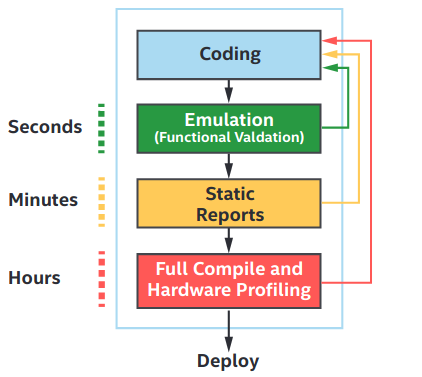
\includegraphics[width=\linewidth]{figures/development-fpga.png}
  \caption{FPGA Development Flow}
    \label{fig:dev}
\end{figure}

There is a perfect pipelining when each stage of the pipeline is occupied and doing useful work every clock cycle as described in Figure \ref{fig:pipeline}.

\begin{figure}[H]
  \centering
  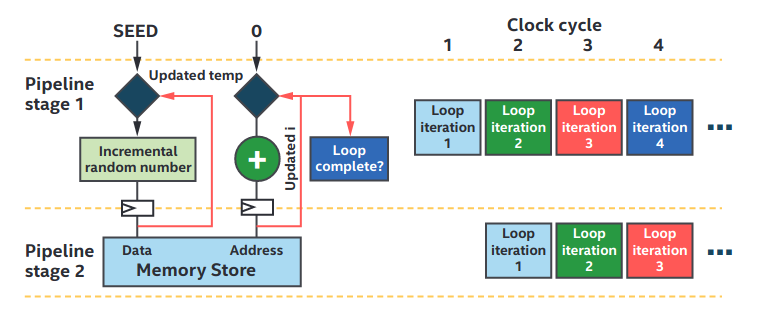
\includegraphics[width=\linewidth]{figures/pipeline.png}
  \caption{Pipeline}
  \label{fig:pipeline}
\end{figure}

However, because a data dependence may require numerous clock cycles to compute in real algorithms, it is frequently not practical to start a new loop iteration every single clock cycle.
When memory lookups, especially those from off-chip memories, are involved in the computation of a dependency, this problem frequently occurs.
As a result, the pipeline has an initiation interval (II) of N clock cycles and can only start a new loop iteration once per N clock cycles.
An II larger than one can lead to inefficiency in the pipeline because
the average occupancy of each stage is reduced. Restructuring the compute in a loop based on the reports can often reduce the II.
Another important concept in spacial architectures is Pipes. They allow us to decompose a problem into smaller pieces to focus on
development and optimizations in a more modular way.

\section{System design}
In this section, we first provide an overview
of the Crystal tile-based execution approach. Then, we detail how we ported it from CUDA to DPC++. Eventually, we describe custom FPGA implementations leveraging that specific accelerator.  

\subsection{Crystal Tile-based Execution Model}
The idea behind tiling comes from the observation that threads in a GPU are grouped into thread blocks (in CUDA terminology) such that threads within a thread block can communicate through the shared memory and synchronize through barriers. Hence, even though a single thread on the GPU at full occupancy can hold only up to 24 integers in shared memory, a single thread block can hold a significantly larger group of elements collectively between them in shared memory. 
The set of data elements that can be collectively processed by a thread block is referred to as a \textbf{tile}. In this fashion, it is possible to design kernels in terms of block-wide device functions dealing with a set of tiles as units of input and output. Each function uses vector instructions for memory accesses, and registers for storing values.

One key advantage of this approach is that after a tile
is loaded into the shared memory, subsequent passes over the
tile will be read directly from shared memory and not from
global memory, avoiding the second pass through global
memory described in the implementation above.

\subsection{DPC++ Porting}
In order to migrate the original CUDA implementation of Crystal to DPC++, we start with Intel's official migration tool, which allows to convert CUDA code to DPC++ at syntax level recognizing the main CUDA constructs and converting them to their DPC++ equivalent. Our goal in using the compatibility tool is to understand and document issues in converting various aspects like data movement, kernel parameterization, atomics and synchronization from CUDA into DPC++,

Using the Compatibility Tool involves the use of the command
dpct that takes a .cu file as input and produces its DPC++ counterpart, with dp.ct extension. Thus, we apply the command to all .cu file of the project. At the source level, the overall translation is quite accurate. dpct automatically adds necessary boilerplate such as headers and compiler directives required for enabling DPC++ compilation. Similarly, dpct preserves and converts templatized functions that correspond to block primitives and join kernels of the Crystal library for most part, with some minor syntactic modifications. At
the programming model level, dpct replaces CUDA kernel launches
with an nd\_range parallel\_for kernel. Further, CUDA data management calls that move data from host to device memory, or assign specific values to device allocated memory regions, are replaced with appropriate DPC++ calls ( memcpy and memset functions of the DPC++ queue class).

Despite its utility, dpct does not convert everything automatically and correctly and the additional porting work to be done by the developer is not negligible. The first issue concerns kernel dimensions. CUDA programming model requires kernel dimensions to be specified in terms of number of threads in a thread block, and the number of thread blocks per grid. Moreover, both thread blocks and grids can be multidimensional. Similarly, DPC++ uses the notion of work-item and work-group. Thus, a CUDA thread block roughly corresponds to a DPC++ work-group, and a CUDA thread gets mapped to a
work-item in DPC++. DPC++ also provides an nd\_item object to
enable index lookup in a nd\_range kernel. It represents the index of each work-item. 
However, despite the fact that the original code implements a 1D kernel, dpct converts it into 3-dimensional kernel. As consequence, all accesses to the threads indexes (local-id, global-id, group-id) within the kernel code were
wrong and needed to be rewritten. Second, synchronization primitives and low-level constructs were not ported correctly. 

The third problematic aspect of dpct comes when it has to deal with CUDA library calls. As a matter of fact, Crystal implementation uses extensively CUB library functions, for various tasks. dpct does not to port CUB function calls automatically, thus the software develper needs manually to replace these with calls to DPC++ functions that are semantically equivalent.

Eventually, in some cases, even when the DPC++ conversion is semantically correct, it might be suboptimal in terms of performance. An example is the call to the memory barrier function. dpct converts it automatically into a memory fence in both global memory and local memory which are very expensive. However, in this specific context, a memory fence in the local memory of each work-group was sufficient. 
Thus, we optimized the code generated by dpct manually and reimplemented CUDA atomic functions like atomicCAS and atomicAdd. Therefore, despite being a rather useful tool, dpct is still far from being an accurate porting tool from CUDA to SYCL. 
\subsection{Projection Design}
We consider two forms of projection queries: one that
computes a linear combination of columns (Q1) and one
involving user defined function (Q2):

\begin{lstlisting}[escapechar=\%]
Q0: SELECT a%$x_1$%+ b%$x_2$% FROM R;
Q1: SELECT %$\sigma(ax_1+ bx_2)$% FROM R; 
\end{lstlisting}

where $x_1$ and $x_2$ are 4-byte floating point values. The
number of entries in the input array is $2^{29}$ . $\sigma$ is the sigmoid function 

$$ \sigma(x) = \cfrac{1}{1 + e^{-x}} $$
which can represent the output of a logistic regression model.

Following crystal's block-wide functions design, we implement a single kernel that does two block loads to load the tiles of the respective columns, computes the projection and eventually does a block store to store it in the result array.

\subsection{Hash Join Design}

The join operator comprises two kernels: a build kernel and a probe kernel. The first one populates the hash table with the tuples of the smaller, build relation. Following crystal's approach, we implement a linear probing strategy with the hash table being implemented as a simple array of slots with each slot containing a key and a payload without any pointers. The probe kernel uses the other relation to search for
matches in parallel. Each thread block loads a tile from the probe table, and each thread computes the local sum for a subset of tile elements that meet the predicate condition. Then, all local values are aggregated in a hierarchical fashion, first for all threads within a block, and then across all thread blocks

\subsection{FPGA Select Design}
The design of the select for FPGA follows the best practices of intel oneAPI\cite{githubOneAPIsamplesDirectProgrammingDPCFPGAReferenceDesignsdbMaster}, in particular for its implementation we used \textbf{unrolled loops} and \textbf{predication}.
By replicating the computational logic inside a loop, the loop unrolling process boosts software parallelism.
Both partial and complete unrolling are possible.
Unrolling loops is a typical technique in an FPGA design to directly trade off on-chip resources for greater performance.
Although increasing the unroll factor speeds up throughput, it also causes increased resource usage, which finally exhausts the available memory (bottleneck).
In our implementation, we discovered that using a fully enrolled loop offers the optimal trade-off.

\begin{figure}[H]
  \centering
  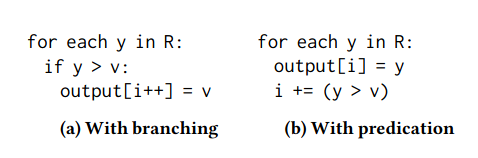
\includegraphics[width=\linewidth]{figures/select.png}
  \caption{Branching vs Predication}
  \label{fig:select}
\end{figure}
An if-statement is used in the branching implementation to carry out the selection.
The penalty for branch mispredictions is the fundamental issue with the branching implementation.
The branch predictor is unable to forecast the branch outcome if the selectivity of the condition is neither too high nor too low.
Performance is hampered as a result of pipeline stalls.
Predication, instead, transforms the branch (control dependency) into a data dependency.
Spatial implementations can communicate results backwards in the pipeline to work that began in a later cycle (i.e., to work at an earlier level in the pipeline) quite well.
By sending outcomes backward in the pipeline, this enables effective data dependence communication.
The ability to pass data backward (to an earlier stage in the pipeline)
is key to spatial architecture \cite{dpcpp_book}.
The main approach that make expressing this pattern easy is through loops.
When a spatial compiler implements a loop, iterations of the
loop can be used to fill the stages of the pipeline.
\subsection{FPGA Hash Join design}
the design of Hash Join on FPGA exploits unrolled loops and \textbf{pipes}.
In our implementation, we discovered that using a fully enrolled loop offers the optimal trade-off.
The producer kernel receives the data from the host memory before sending it over a pipe to the join kernel, which builds the hash table and then performs the join over the probe table and eventually the consumer kernel writes the final result to the host memory. 
Figure \ref{fig:desugnjoin} illustrates the high-level implementation design.
\begin{figure}[H]
  \centering
  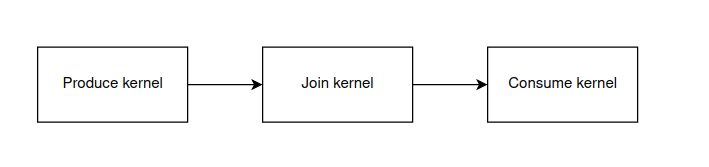
\includegraphics[width=\linewidth]{figures/design-hashjoin-fpga.png}
  \caption{Design Hash Join}
  \label{fig:desugnjoin}
\end{figure}

\section{Operators GPU vs CPU vs FPGA}
In this section, we compare the performance of foundamental SQL operators - project, select, and hash join - on GPU, CPU and FPGA with the goal of understanding how the very same block-functions based implementation works on CPU, GPU, iGPU and how the custom implementation for FPGAs behaves. We will, also, extend the camprison to NVidia hardware targetted via DPC++ and hipSYCL \cite{hipsycl}.

\subsection{Projection on CPU and GPU}
In this section, we will show and comment the results of the projection operator on Intel's and NVidia's hardware, using the design described in \textbf{section 3.3}, with a two-columns table of size $2^{29}$, which is the same study case presented in the original publication \cite{crystal}.

\begin{figure}[H]
  \centering
  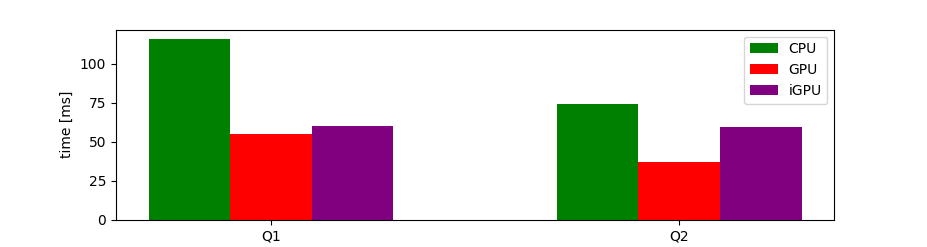
\includegraphics[width=\linewidth]{figures/project_intel.png}
  \caption{Project benchmarks on CPU, GPU and iGPU}
    \label{fig:proj-intel}
\end{figure}

Figure \ref{fig:proj-intel} shows the runtime of
queries Q1 and Q2 on Intel's CPU, GPU and iGPU (shown as bars). The performance of Q1
is memory-bandwidth bound. GPU performs substantially better than the CPU implementation, due to its much higher memory bandwidth and slightly better than the iGPU. 

\begin{figure}[H]
  \centering
  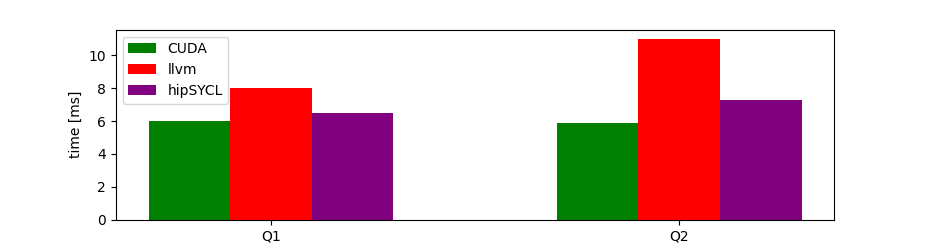
\includegraphics[width=\linewidth]{figures/project_nvidia.png}
  \caption{Project benchmarks on NVidia GPU}
    \label{fig:project-nvidia}
\end{figure}

Figure \ref{fig:project-nvidia} shows the results of the performed benchmarks using the very same setup but on NVidia GPUs, comparing hipSYCL, Intel's llvm and the original CUDA code.

We notice how for both the queries we achieve similar performances and the ported SYCL code is only 5\% slower than the original CUDA code. In addition, hipSYCL yields slightly better performances than the cross-compiled code with llvm.

\subsection{Hash Join on CPU and GPU}

\begin{figure}[H]
  \centering
  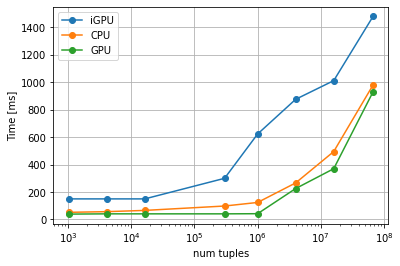
\includegraphics[width=\linewidth]{figures/bench-gpu-cpu.png}
  \caption{Hash Join benchmarks on CPU, GPU and iGPU}
    \label{fig:join-intel}
\end{figure}

\begin{figure}[H]
  \centering
  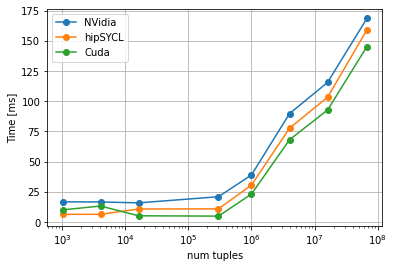
\includegraphics[width=\linewidth]{figures/bench-hip-nvidia-cuda.png}
  \caption{Hash Join benchmark on NVidia GPU}
    \label{fig:join-nvidia}
\end{figure}

We study the Hash Join by focusing on the following
microbenchmark query and configurations that are also used in the original Crystal publication and other prior literature\cite{crystal}.

\begin{verbatim}
    SELECT SUM (A.v * B.v) FROM A, B WHERE A.k = B.k;
\end{verbatim}
where tables A and B consist of two 4-byte integer columns k, v joined on key k. The size of the probe table is fixed at 256
million tuples, totaling 2GB of raw data. We use a hash table with 50\% fill rate and vary the size of the build table such that it produces a hash table in the range 8KB-512MB. After fine-tuning the number of work-items-per-group, we fix this value to 128 both for the CPU and the GPU. 
Figure \ref{fig:join-intel} shows the actual execution time of the probe kernel on Intel's CPU vs GPU vs iGPU for various build table sizes. Differently from prior work in Crystal, where only the probe time was benchmarked, we report the whole execution time, which includes the build time and the allocation time. 

Looking at Figure \ref{fig:join-intel}, we see that the execution time increases twice, namely every time the hash table exceeds the size of the cache (L2 and L3).  for instance, for the CPU these thresholds are 256 KB and 12 MB.

Figure \ref{fig:join-nvidia} demonstrates the comparison of the original Crystal CUDA implementation with the cross compiled version using Intel's llvm and the open-source hipSYCL toolchain, using a work-size of 256. 
Despite improving signifincatly with respect to Intel's discrete GPU, these results show that cross-compiled implementation is less efficient than the native implementation, which outperforms the cross-compiled one of 1.4 times so that there is room for further improvement.

However, considering the fact that the DPC++ implementation has
the advantage of being executable on Intel® GPU and multicore
CPU with no change in kernel code except for kernel dimensioning, we believe that trading off performance to achieve portability is one worth a serious consideration.

\subsection{Evaluation of Operators in FPGA}
Our experiments were conducted on Intel® DevCloud and we performs benchmarks of hash join and select operator on Intel® Arria and Intel® Strattix. We also calculated the Global Memory Bandwidth Usage.
The LSU(Load Store Unit) bandwidth equation is the minimum of three bottlenecks we need to calculate the use of global memory bandwidth \cite{fpga_optim}. These formulas represent the theoretical maximum bandwidth an LSU may consume
\begin{equation}
\label{eqn:bandwidth}
\text{LSU bandwidth} = min\{BW_1, BW_2, BW_3\} \ \text{MB/s}
\end{equation}
$$ \text{BW1} = k_{width} \cdot f_{max} $$
$$ \text{BW2} = m_{width} \cdot f_{max} $$
$$ \text{BW3} = \frac{\text{BW}_{\text{max}} \cdot N^{i}_{ch}}{N_{ch}}$$
where $k_{width}$ represent the byte-width of the LSU on the kernel, $m_{width}$ represent the byte-width of the LSU facing the external memory, $f_{max}$ is the clock-speed of the kernel in MHz, $\text{BW}_{\text{max}}$ is the Maximum Bandwidth the global memory can achieve, $N_{ch}$ represent the number of interfaces and external memory has and $N^{i}_{ch}$ assume the same value of the number of channels if interleaving is enabled, otherwise is 1.


\subsection{FPGA Select}
We use the following micro-benchmark to evaluate selections:
\begin{verbatim}
SELECT y FROM R WHERE y < v;
\end{verbatim}    
where we vary the selectivity of the predicate from 0.1 to 1.
The input table is composed of two columns of 32-bit integer, for our evaluation we generate a table of $2^{28}$ rows.
The entire input array is scanned and written to the output array. The measured runtime - only for load/store from host memory to device memory and vice versa - can be computed as follows
$$runtime = \frac{8 N}{B_r} + \frac{8 N}{B_w}$$
where $B_r$ represent the bandwidth for the load, $B_w$ represent the bandwidth for the store while $N$ is the number of rows.
By looking at the report generated, it were used two LSUs for the load and two LSUs for the store.
On Intel® Arria, the estimated Frequency is 240 MHz, therefore plugging into Equation \ref{eqn:bandwidth}, we end up with a measured bandwidth of 2224 MB/s for the load and 2224 MB/s for the store

Table \ref{tab:select-arria} shows detailed results on the Total latency and kernel time.
\begin{table}[H]% h asks to places the floating element [h]ere.
  \caption{Evaluation on Intel Arria 10 GX}
  \label{tab:select-arria}
  \begin{tabular}{cccl}
    \toprule
    Selectivity & Total latency[ms] & kernel time[ms]\\
    \midrule
    0.1 & 2786& 967.8\\
    0.2 & 2781.2 & 967.8\\
    0.4 & 2762.6 & 967.8\\
    0.6 & 2787.9 & 967.8\\
    0.8 & 2786.4 & 967.8\\
    1 & 2785.3 & 967.8\\
  \bottomrule
\end{tabular}
\end{table}
We conclude that $70\%$ of the total latency is spent to load and store from the host memory to the device memory and vice versa.

Reproducing the very same benchmarks on Intel® Strattix FPGA board, where the estimated Frequency is equal to 432 MHz, using Equation \ref{eqn:bandwidth}, we obtain a measured bandwidth of 2872 MB/s for the load and 2872 MB/s for the store, so the time spent only for the load and store is 1495 ms, less than Intel® Arria but still corresponding to the $60\%$ of the total latency.
Table \ref{tab:select-strattix} shows detailed results of the total latency and kernel time.
\begin{table}[H]% h asks to places the floating element [h]ere.
  \caption{Evaluation on Intel Strattix 10 SX}
  \label{tab:select-strattix}
  \begin{tabular}{cccl}
    \toprule
    Selectivity & Total latency[ms] & kernel time[ms]\\
    \midrule
    0.1 & 2310& 749.0\\
    0.2 & 2316.66 & 749.0\\
    0.4 & 2311.48 & 749.0\\
    0.6 & 2311.66 & 749.0\\
    0.8 & 2316.7& 749.0\\
    1 & 2298.66 & 749.0\\
  \bottomrule
\end{tabular}
\end{table}
For the sake of completeness, Table \ref{tab:area-select} also reports the results on the use of the available area.
\begin{table}[H]% h asks to places the floating element [h]ere.
  \caption{Area analysis}
  \label{tab:area-select}
  \begin{tabular}{cccl}
    \toprule
     & ALUTs & RAMs & DSPs\\
    \midrule
    Static Partition & 179950 (21\%) & 492 (18\%)  & 123 (8\%)\\
    Kernel System & 5897 (1\%)  & 89 (3\%)  & 0 (0\%)\\
  \bottomrule
\end{tabular}
\end{table}

\subsection{FPGA Hash Join}
In this section we will evaluate the performances of the DPC++ Hash join implementation running on Intel Arria® 10 GX and Intel Strattix 10 SX and then compare them with the previous benchmarks obtained on Intel CPU and discrete GPU. We use the following micro-benchmark to evaluate the operator:
\begin{verbatim}
SELECT R.k, R.v, S.k, S.v FROM R, S WHERE R.k = S.k;
\end{verbatim}
where R and S are two-columns table of 32-bit integer.
Due to kernel memory restrictions, we keep fixed the Build table to have size of 2 MB ($2^{18}$ rows) and we vary the size of the the Probe table.
The entire Probe table and Build table are read and then only the joined rows are written to the output array, thus having 3 columns (key, value\_build\_table, value\_probe\_table). The measured runtime, only taking into account load/store from host memory to device memory or vice versa, in the worst case scenario, is equal to
$$runtime = \frac{8 P + 8 B}{B_r} + \frac{12 P}{B_w}$$
where $B_r$ represent the bandwidth for the load, $B_w$ represent the bandwidth for the store, $P$ is the number of rows of the Probe table and $B$ is the number of rows of the Build table.
The produced report shows that 4 LSUs have been employed for  the load and 3 LSUs for the store.
Taking into that that the estimated frequency on Intel® Arria is equal to 240 MHz, using Equation \ref{eqn:bandwidth}, we obtain a measured bandwidth of 3536 MB/s for the load and 2652 MB/s for the store.
Table \ref{tab:join-arria} shows the results of the benchmarks on Intel® Arria.
\begin{table}[H]% h asks to places the floating element [h]ere.
  \caption{Evaluation on Intel Arria 10 GX}
  \label{tab:join-arria}
  \begin{tabular}{cccl}
    \toprule
    Probe Table size & Total latency[ms] & kernel time[ms]\\
    \midrule
    8kB & 46.7& 1.01\\
    32kB & 45.98 & 1.05\\
    128kB & 45.67 & 1.00\\
    3MB & 47.8 & 2.39\\
    8MB & 51.2 & 4.76\\
    32MB & 85.2 & 19.03\\
    128MB & 222.29 & 76.10\\
    512MB & 805.6 & 304.3\\
  \bottomrule
\end{tabular}
\end{table}
We notice that, on average, $40\%$ of the time is spent for load and store operations.
Generating the report for Intel® Strattix instead, the estimated frequency is 349.92 MHz, so doing similar calculations as before , we obtain a measured bandwidth of 5392 MB/s for the load and 4044 MB/s for the store.
Table \ref{tab:join-strattix} shows the results on Intel® Strattix.
\begin{table}[H]% h asks to places the floating element [h]ere.
  \caption{Evaluation on Intel Strattix 10 SX}
  \label{tab:join-strattix}
  \begin{tabular}{cccl}
    \toprule
    Probe Table size & Total latency[ms] & kernel time[ms]\\
    \midrule
    8kB & 56& 0.65\\
    32kB & 56.8 & 0.60\\
    128kB & 56.5 & 0.61\\
    3MB & 55.1 & 1.56\\
    8MB & 55.48 & 3.12\\
    32MB & 84.1 & 12.47\\
    128MB & 198.8 & 49.84\\
    512MB & 635.4 & 200\\
  \bottomrule
\end{tabular}
\end{table}
Similarly to Arria, we conclude that on average $40\%$ of the time is spent performing load and store operations.
Table \ref{tab:area-join} reports the area usage of the device.
\begin{table}[H]% h asks to places the floating element [h]ere.
  \caption{Area analysis}
  \label{tab:area-join}
  \begin{tabular}{ccccccl}
    \toprule
     & ALUTs  & RAMs & DSPs\\
    \midrule
    Static Partition & 466792 (25\%) & 3039 (26\%)  & 1291 (22\%)\\
    Kernel System & 29053 (2\%)  & 1556 (13\%)  & 0 (0\%)\\
  \bottomrule
\end{tabular}
\end{table}
Finally, Figure \ref{fig:fpga-cpu-gpu} shows a summary plot comparison of the FPGAs benchmarks against Intel® Iris® Xe MAX Graphics (dGPU) and Intel® Xeon® Gold 6128 CPU.
\begin{figure}[H]
  \centering
  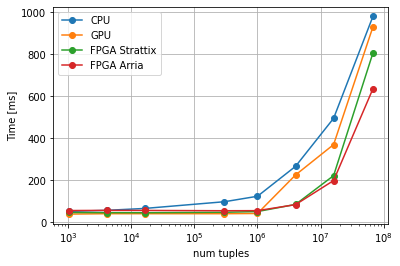
\includegraphics[width=\linewidth]{figures/bench-fpga-gpu-cpu.png}
  \caption{Benchmarks on FPGAs, GPU, CPU}
  \label{fig:fpga-cpu-gpu}
\end{figure}



\section{WORKLOAD EVALUATION}
Now that we have a good understanding of how individual operators perform on CPU, GPU and FPGA, we will evaluate the performance of a workload of full SQL queries on these
hardware platforms. 
We first describe the query workload we use in our evaluation. We then present a high-level comparison of the performance of queries implemented with the tile-based execution model running on Intel's CPU, GPU and iGPU versus Nvidia GPU. We also report the performance of the original CUDA implementation of crystal. In addition, we propose a comparison with the performances yield on NVidia Hardware compiled with the open-source hipSYCL\cite{hipsycl} runtime. 
% As a case study, we provide a detailed
%performance breakdown of one of the queries to explain
%the performance gains. 
%Finally, we present how the very same code performs when used to %target an FPGA board for a single query. 

For experiments run on Intel Hardware, including FPGAs, we use Intel's devcloud platform. For experiments run on
Nvidia GPU, we use an machine equipped with an Nvidia NVIDIA GeForce RTX 2080 Ti
GPU, CUDA 11.4 and running on Ubuntu 20.04. In our evaluation, we
ensure that data is already loaded into the respective device’s
memory before experiments start. We run each experiment 3 times and report the average measured execution time


\subsection{workload}
For the full query evaluation, we use the Star Schema Bench-mark (SSB) \cite{ssb}, a simplified version of the more popular TPC-H benchmark. It has one fact table lineorder and four dimension tables date, supplier, customer, part which are organized in a star schema fashion.
There are a total of 11 queries in the benchmark, divided into 4 query flights. 
In our experiments we run the benchmark with a scale factor of 20 which will generate the fact table with 120 million tuples. The total dataset size is around 13GB.


\subsection{performance comparison}

\begin{figure*}
    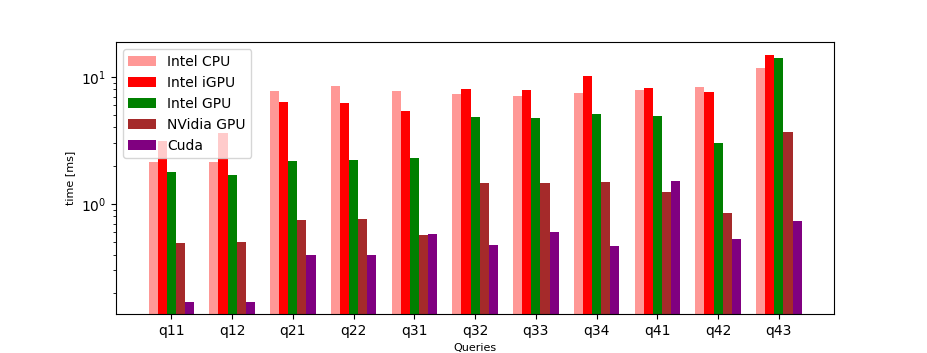
\includegraphics[height=.33\textheight, width=1\linewidth]{figures/queries.png}
    \caption{Star Schema Benchmark Queries}
    \label{fig:ssb}
\end{figure*}
In order to ensure a fair comparison across systems, we dictionary encode the string columns into integers prior to data loading and manually rewrite the queries to directly reference the dictionary-encoded value, as done in crystal. 
For example, a query with predicate s\_region = ‘ASIA’ is rewritten with predicate s\_region = 2, where 2 is the dictionary-encoded value
of ‘ASIA’. 
However, in our benchmark we make sure all column entries
are 4-byte values to ensure ease of comparison with other
systems and avoid implementation artifacts. 
We use a thread block size of 128 with tile size
of 4 (= 4×128) resulting in 4 entries per thread per tile.
The results are shown in Figure \ref{fig:ssb}. 
We can notice how the NVidia GPU significantly outperforms Intel's hardware with the same implementation, resulting on average in a 3.5x speedup with respect to the discrete GPU and a 5.8x speedup with respect to the CPU. 
Nevertheless, the original CUDA implementation of crystal shows on average a 1.9x speedup with respect to the SYCL porting, with the latter one outperforming the first one for some queries. 



\begin{figure*}
    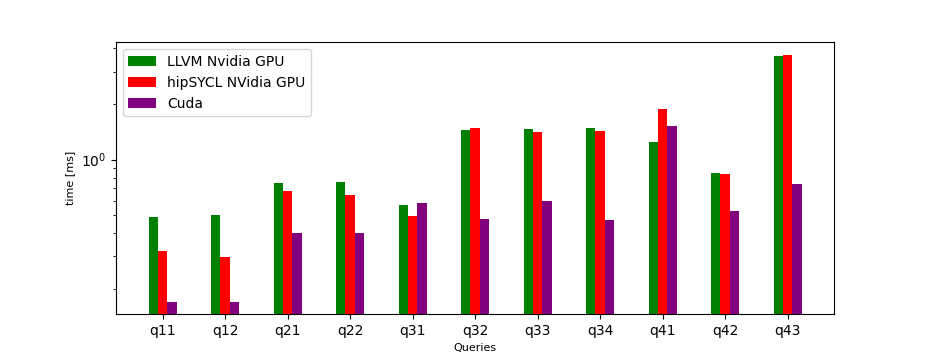
\includegraphics[height=.33\textheight, width=1\linewidth]{figures/queries_hipsycl.png}
    \caption{Star Schema Benchmark with hipSYCL}
    \label{fig:hipsycl}
\end{figure*}

The further comparison with hipSYCL is shown in Figure \ref{fig:hipsycl}. We can notice a speedup for smaller queries, but on average both llvm and hipSYCL show similar performances with just a 0.01 mean discrepancy.  

\section{Conclusion and Future Works}
Developing applications that are performance-portable has been a
major challenge in the HPC world, and we believe that lack of performance portability is one of the main reasons hindering a much broader adoption of XPU by data management systems. Our work shows that single-source, cross-architecture programming models like DPC++ are a step in the right direction, which opens up several other lines of future research.

On the runtime front, more work is required to understand the gap in performance between DPC++ and other optimized, proprietary platforms like CUDA.


ref{fig:fpga}.
\begin{figure}[H]
  \centering
  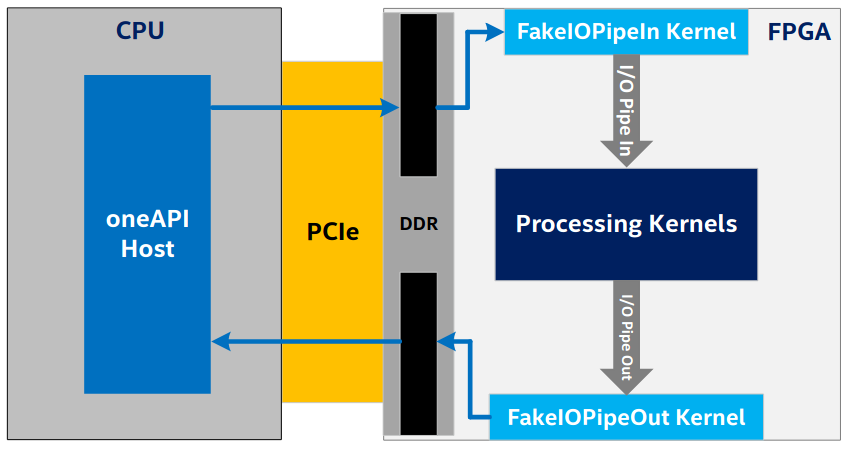
\includegraphics[width=\linewidth]{figures/FPGA.png}
  \caption{FPGA architecture}
  \label{fig:fpga}
\end{figure}

On the FPGA front, we conducted an analysis aiming at comparing its performances with CPUs and GPUs. Based on these analysis, we showed that major obstacle for accelerating DBMS operators on the FPGA is the memory bandwidth as also pointed out by \cite{Chen2020IsFU}. The widely used CPU-FPGA platforms are usually discrete, in which an FPGA board with private memory resource is attached via PCIe
bus as a peripheral of the CPU, as shown in Figure \
The compiler instantiates a specialized LSU for each access site based on the
memory access pattern to maximize the efficiency of data accesses.
All accesses to global memory must go through the hardware interface. The compiler
connects every LSU to an existing hardware interface through which it transacts with
device global memory. Since the compiler cannot alter that interface or create more
such interfaces, it must share the interface between multiple datapath reads or writes,
which can limit the throughput of the design \cite{fpga_optim}.
The strategies used by the compiler to
maximize efficient use of available memory interface bandwidth include (but are not
limited to) the following:
\begin{itemize}
    \item  Eliminating unnecessary accesses.
    \item Statically coalescing contiguous accesses.
    \item Generating specialized LSUs that can perform the following:
    \begin{itemize}
        \item Dynamically coalesced accesses that fall within the same memory word (as
defined by the interface)
\item Prefetch and cache memory contents
    \end{itemize}
\end{itemize}
In this architecture, before any computation on the FPGA can start, the CPU must copy the data to the FPGA's private memory through the PCIe bus and copy the results back after the computation is finished.
Therefore, data transport and/or synchronization overhead typically place limits on speed improvements.
Tightly coupled CPU-FPGA designs have been developed to pro-
vide memory coherency between CPU and FPGA in order to reduce
communication latency and reduce data transmission overhead. For
example, Intel started the Hardware Accelerator Research Program
(HARP)\cite{harp}. So it would be interesting in the future to explore this
Architecture and repeat the same benchmarks and comparing it with a stateof-the-art FPGA-based join implementation\cite{FPGAbasedMF}.
However, FPGAs are a cheaper off-the-shelf alternative that you can reprogram for each new application, while a custom ASIC even if generally outperforms an FPGA on a specific task, they take significant time and money to develop.

%\clearpage

\bibliographystyle{ACM-Reference-Format}
\bibliography{sample}

\end{document}
\endinput
